\chapter{Introduction}
\label{ch:introduction}

\section{Motivation}

The content seen on social media varies greatly from user to user. This is because social media use recommender systems to
show users content they are likely to be ``interested" in \cite{}. These recommender systems are based on a users past interactions \cite{}
Typically, if a user views a certain type of post, they are likely to view similar posts in the future. This project aims
to find the interests of a user by analysing their social media posts.\\

Take a look at the following example:
\begin{figure}
    \centering
    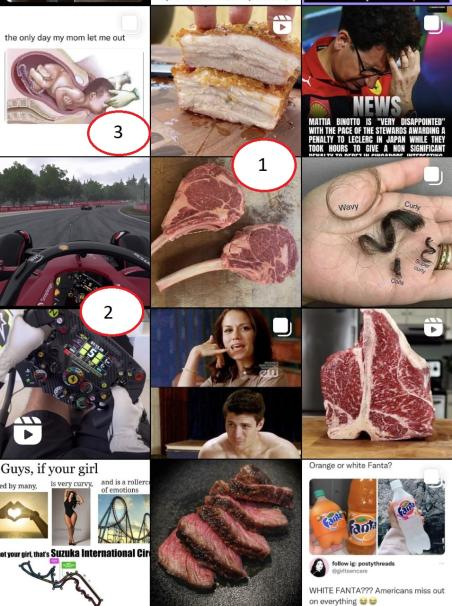
\includegraphics[width=0.6\textwidth]{../images/tweet-example.png}
    \caption{Example tweet}
    \label{fig:motivation-example}
\end{figure}

This set of social media posts are taken from a user's social media feed. As a human, we can easily identify what the user is
interested in; they are interested in Formula 1 and Food (specifically, steak). We make this assumption based on the content
of the posts.\\

Looking at the posts, there rises a couple questions:
\begin{itemize}
    \item What are the posts about?
    \item Are the posts seen representative of all posts across the social media platform?
    \item How can users find other posts that are dissimilar to the posts they are shown?
\end{itemize}

\subsection{Topics}
This project will use the notion of topics to identify what the posts are about.
\begin{figure}[hbtp]
    \centering
    a subject that is discussed, written about, or studied
    \caption{Topic Definition - \cite{cambdict}}
    \label{fig:topic_definition}
\end{figure}

This definition of a topic is a good starting point for this project. This definition is a bit too specific. If this definition were 
to be used there would be no meaningful output from this project - due to the fact you could classify each post into its own unique
topic. To overcome this, we will use a more general definition of a topic. Essentially, a topic comprises of a set of words that
are related to each other.

\subsection{Problem Statement}
The goal of this project is to be able to classify social media posts. This will allow us to identify interests through comparing
similarities between posts shown to the user. This will be followed by quantifying a set of posts to compare the similarity between
a users posts and posts from the entire social media site. Finally, this project aims to create a user interface that allows users
to discover what their social media feed says about their interests and how they compare to the rest of the social media site. The
user interface will also allow users to discover posts that are dissimilar to the posts they are shown.


\section{Related work}
\subsection{Pythia - \cite{Pythia}}
\label{sec:pythia}
Pythia is an automated system for short text classification. It makes use of Wikipedia structure and articles to identify
topics of posts.
Essentially, "Wikipedia contains articles organized in various taxonomies, called categories". Pythia then goes on to use
this information as their training data as well as handling sparseness in posts on social media.\\

Pythia also demonstrates a method to overcome the lack of context in short texts - This is a large problem in identifying
smaller social media posts like tweets, and will be further worked on in this project. They use a method called "Post Enrichment",
which performs i) Named Entity Recognition then ii) Lemmatization and stop word removal. We then use the named entities to query
wikipedia for similar articles that are then appended to the post.\\

Although this method works well in cases where keywords are used, there are cases where no keywords are used, and more context
is needed. Take for example the following tweet:
\newpage
\begin{figure}[htbp]
    \centering
    
\includegraphics[width=0.6\textwidth]{../images/tweet-example2.png}
    \caption{Example tweet}
    \label{fig:tweet-example}
\end{figure}

The text gives us very little context; What is this tweet about? the best guess I could give
is it is a message to other users. If these users had wikipedia articles, we could use them. But in reality this post is about something else.
Lets add some other form of context; add the media the tweet contains.
\begin{figure}
    \centering
    
\includegraphics[width=0.6\textwidth]{../images/tweet-media.png}
    \caption{Example tweet - media}
    \label{fig:tweet-media}
\end{figure}
This gives us a lot more context; the tweet is discussing the earthquake that hit Turkey and Syria, if we use this for our query we get more relevant
articles:
\newpage

\begin{figure}[htbp]
    \centering
    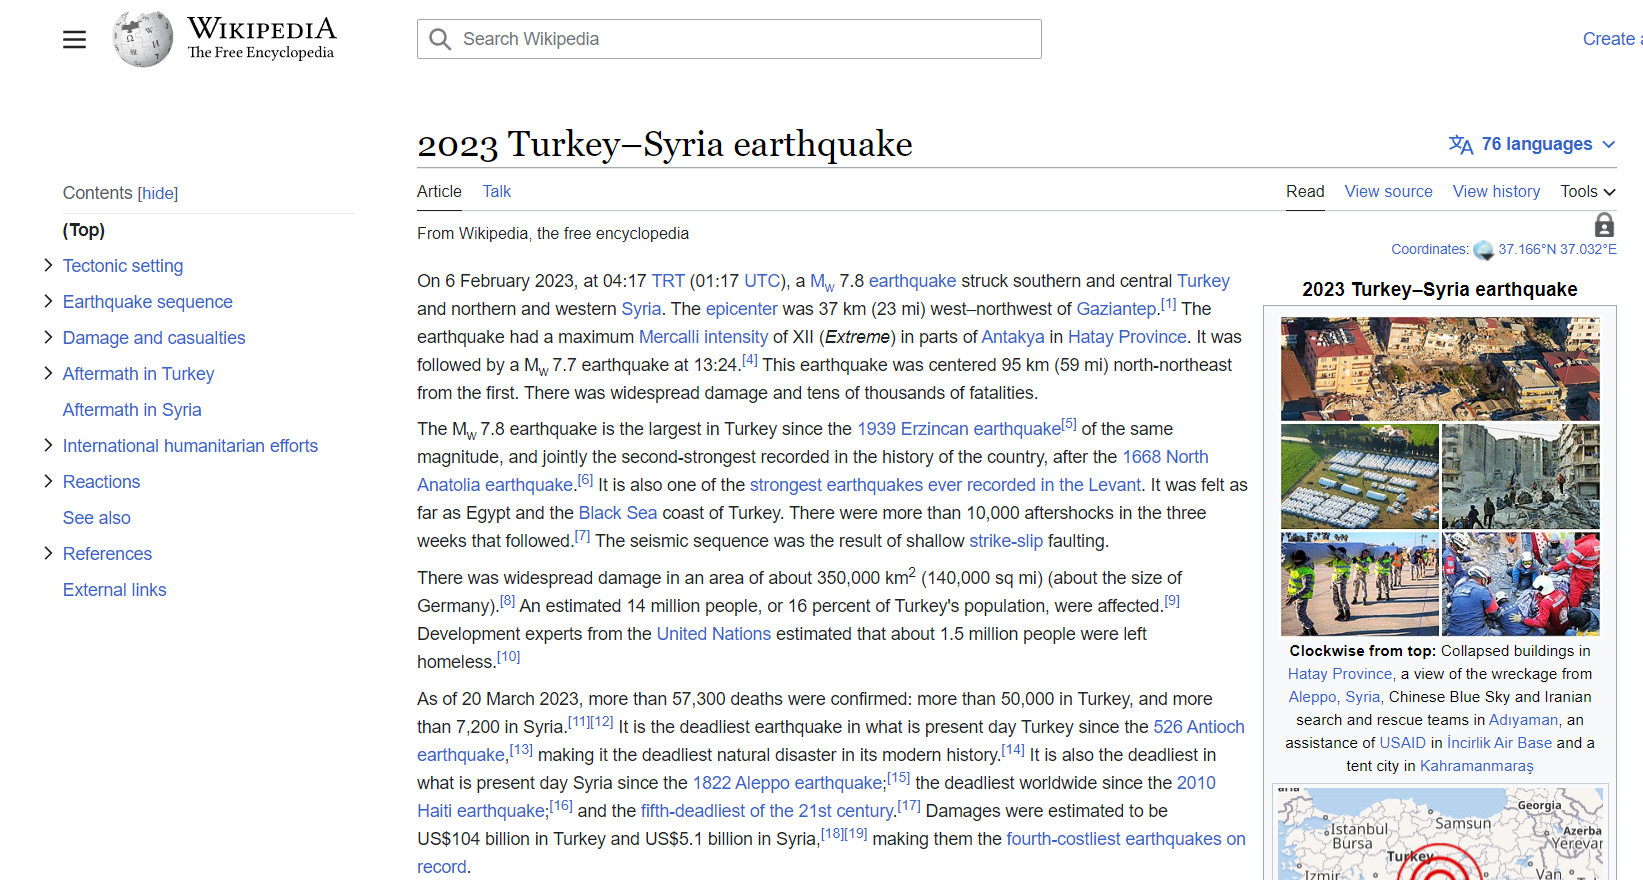
\includegraphics[width=0.6\textwidth]{../images/post-context-example.png}
    \caption{Wikipedia articles related to the hashtag "BLASTPremier"}
    \label{fig:blastpremier}
\end{figure}

We now have a lot of relevant information to append to the post. We could use other information for context as well: Tweet author,
images/media in tweets, retweet information, like information, etc.

\subsection{Topic tracking of student-generated posts - \cite{TopicTracking}}
This paper proposes a solution for determining valuable information/topics discussed in student forums on online courses.
It uses a model called "Time Information-Emotion Behaviour Model" or otherwise called "TI-EBTM" to detect key topics discussions
, keeping in mind the progress of time throughout the forum.\\
Although this paper specializes in academic online forums, the approaches made could be relevant and useful for this project.

\subsection{Topic classification of blogs - \cite{husby2012topic}}
This paper uses Distant Supervision - 'an extension of the paradigm used by (\cite{snow}) for exploiting WordNet to extract hypernym (is-a) relations between entitities'
- to get training data via Wikipedia articles. Then trains their own designed model on this data to be able to classify topics via a
multi-class recognition model (69\% accuracy) and via a binary classification model (90\% accuracy).

\section{Objectives}
To achieve the problem statement, the following objectives must be met:
\begin{itemize}
    \item Generate a list of topics for classification
    \item Implement methods for identifying the topics in social media posts
    \item Compare and contrast the results of the different methods
    \item Create a user interface
    \begin {itemize}
        \item Allow users to compare their interests to the rest of the social media site
        \item Allow users to discover posts that are dissimilar to the posts they are shown
    \end{itemize}
\end{itemize}
The largest problem with this project is the second objective of finding and creating methods for identifying topics.